\chapter{METHODOLOGY}
\label{chp:methodology}

\todo{write}

\section{Approach Overview}
\label{sec:approach-overview}
\todo{write}
buraya akış şeması çiz

\section{Process Model Mining}
\label{sec:process-model-mining}
Process model mining stage in the proposed approach has the aim of creating reproducible and generalized process models from event logs. In order to achieve this aim, implementation of \textit{Inductive Miner Infrequent (IMi)}, which is proposed in \cite{leemans2014discoveringinfrequent} as an extension to \textit{Inductive Miner} to handle noise in the event logs, is used in this study. 
The selected implementation has the ability of pruning data to handle noise in the event logs. Like the other data mining approaches, event logs include data related to the infrequent behaviors occurred in real life. Although these infrequent behaviors might be caused by important structural or case related issues that should be analyzed; they make the process of mining and results more complex. In the scope of this study, without cleaning the data, most of the process model mining approaches result with \textit{spaghetti-like models}\cite{van2011process} which are difficult to further analyze. Since this thesis focuses on learning from the cross-organizational process mining rather than creating the best-fitting process models, data cleaning and noise handling is a necessary step. Therefore preprocessing steps are undertaken with a compatible approach of \textit{Inductive Miner Infrequent (IMi)}, where data is cleaned in every inductive step.
Considering the scope of this study, instead of computational details of \textit{Inductive Miner Infrequent (IMi)} black-box approach is used to explain its usage in the methodology. In order to provide a filtering threshold, a user-provided value between 0 to 1 is added as input to method with the event logs. As a result, workflow net is produced which is a sound and properly completed Petri net without deadlocks. Black-box of this stage is illustrated in Figure~\ref{fig:process-model-mining-blackbox} and this stage is called for every organization's event logs to create their own process models in Workflow net formalization.

\begin{figure}
  \centering
  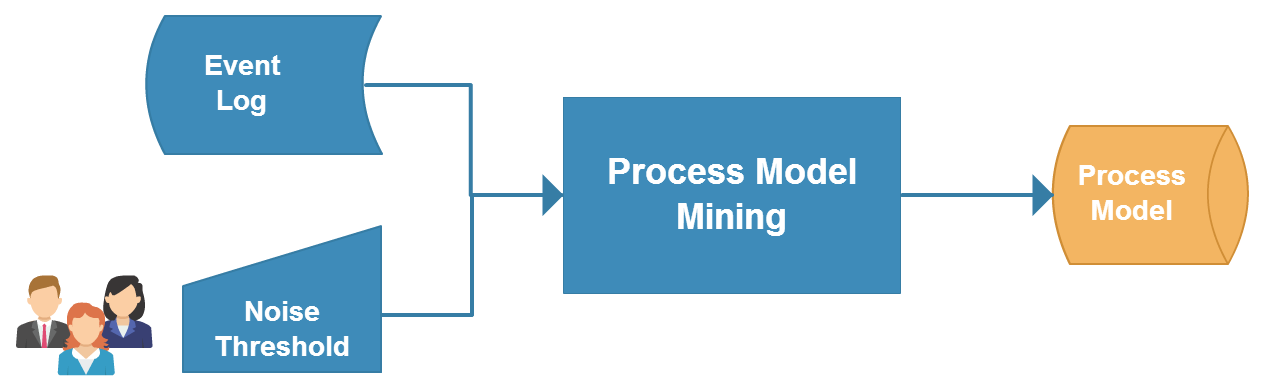
\includegraphics[width=\textwidth]{4_methodology/process-model-mining-blackbox}
  \caption{Process Model Mining Stage as Black-box }
  \label{fig:process-model-mining-blackbox}
\end{figure}


\section{Performance Indicator Analysis}
\label{sec:performance-indicator-analysis}
Performance indicator analysis stage focuses on calculating and analyzing the performance values using the event logs and mined process models. This stage consists of mainly two concepts as 
\begin{inparaenum}[\itshape a\upshape)]
\item alignment and calculation of performance indicators; and
\item clustering of organizations based on their performance values.
\end{inparaenum}
In order to evaluate the performance of an organization based on their process models and past activities; there are a number of indicators in time dimension, cost dimension and utilization \cite{van2011process}. However, in this study, process related performance values are considered since differences in the process models are studied in the next stages. With this reasoning, the following performance indicators are calculated and analyzed in this stage of methodology:
\begin{description}
  \item[Average Time Between Activities] For each activity in the process model, average time to reach other activity is calculated. This is a simple but powerful performance metric for organizations since it can yield the average time to complete one task based on a starting point. From the performance perspective, organizations want to minimize average time between activities to increase their throughput \cite{van2012replaying}. This notion can be defined as following:
\theoremstyle{definition}
\begin{definition}{}
$AvgTime_{Activity_{A}\rightarrow Activity_{B}}^{Organization_{i}} = \frac{\sum_{Case\ c \in Event Log_{i}} EndTime_{c}(Activity_{B}) - StartTime_{c}(Activity_{A})}{Occurences_{Event Log_{i}}(Activity_{A}, Activity_{B})}
$ where
\begin{enumerate}
\item $StartTime_{c}(Activity_{A})$ means start time of $Activity_{A}$ in $Case c$.
  \item $EndTime_{c}(Activity_{B})$ means end time of $Activity_{A}$ in $Case c$.
  \item $Occurences_{Event Log_{i}}(Activity_{A}, Activity_{B})$ means the number of occurrences of  $Activity_{A}$ followed by  $Activity_{B}$ in  $Event Log_{i}$.
\end{enumerate}
\end{definition}

  \item[Standard Deviation of Time Between Activities $StdDevTime_{A\rightarrow B}^{Organization_{i}}$] Time between activities in real life is not stable and they deviate due to various reasons such as people responsible of tasks, size and the content of tasks or seasonality \cite{van2011process}. On the other hand, organizations want to be confident about their processes and therefore they want to minimize the deviation in the time between activities. Minimized deviation in time helps organizations to plan, act and re-organize the activities in the processes with high accuracy \cite{van2012replaying}.
\end{description}
In addition to average and standard deviation, minimum and maximum times between activities can also be analyzed. However, these performance values are mostly result of rare cases in the event logs and these rare occurrences have the probability of being eliminated as noise in process mining stage. Therefore, the minimum and maximum values have the risk of not representing the actual performances. Thus, only average and standard deviation of the time between activities are selected in the study. 

\subsection{Replay and Performance Indicator Calculation}
\label{subsec:replay-and-performance-summary}
Replay of event logs on process models is based on the idea of \textit{alignment} which is formalized in \cite{van2012replaying} and the basic assumption in this concept is that process models and event logs have the same activity labels. Alignment is based on \textit{moves in the model and log} and in order to have a successful replay, optimal alignment should be achieved. As proposed in \cite{adriansyah2011conformance} \cite{adriansyah2011towards}, $A^{*}$ algorithm which is a path-finding algorithm based on graphs is used to find optimal alignment of event logs on the process models.
In order to appropriately apply $A^{*}$ algorithm, there are number of manual and computational steps that should be undertaken. The following prerequisite steps are implemented in \cite{adriansyah2011towards} to apply $A^{*}$ algorithm:
 \begin{description}
	\item[Set Label Patterns between Process Model and Event Log:] In order to match all activities in the event log, user input is necessary to match different transitions in the event logs to the activities in the process models. For instance, there can be \textit{"Activity A, Start"} and \textit{"Activity A, End"} in the event log; however they are reflected as \textit{"Activity A"} in the process model. Therefore, a list of all transitions and events are asked to the user to match to the ones in the process model.
	\item[Create Initial and Final Markings:] In the case of there is no definite starting or ending point in the process model, user input is necessary to define these activities.
	\item[Set Cost Values:] Since $A^{*}$ algorithm is based on alignments which are basically moves along process models and event logs, cost values for each move is necessary to be set. Cost assignment is necessary for the following moves:
	\begin{inparaenum}[\itshape a\upshape)]
		\item move on process model, 
		\item move on event log; and
		\item synchronous move.
	\end{inparaenum}
\end{description}
In order to use replay as an intermediate stage in this thesis, some of the mentioned steps are automatized with the help of the assumptions in the prior and post stages of methodology. With this reasoning, initial and final markings are created with the first and last activities in the process models. In addition, since there is no explicit priority of process model over event log or vice versa, cost values are set to 1 for both \textit{move on process model} and \textit{move on event log}. Since there is no penalty for \textit{synchronous moves}, their cost value is set to 0. However, since each event log has different set of transition labels, manual user input is still necessary to map label patterns between process model and event log. With the user inputs and generated inputs, usage of replay and performance indicator calculation in the methodology can be visualized in Figure~\ref{fig:replay-and-performance-indicator-calculation}. For each organization, the steps in the diagram are followed with the corresponding event logs and process models, resulting process summaries are used for further analysis.

\begin{figure}
  \centering
  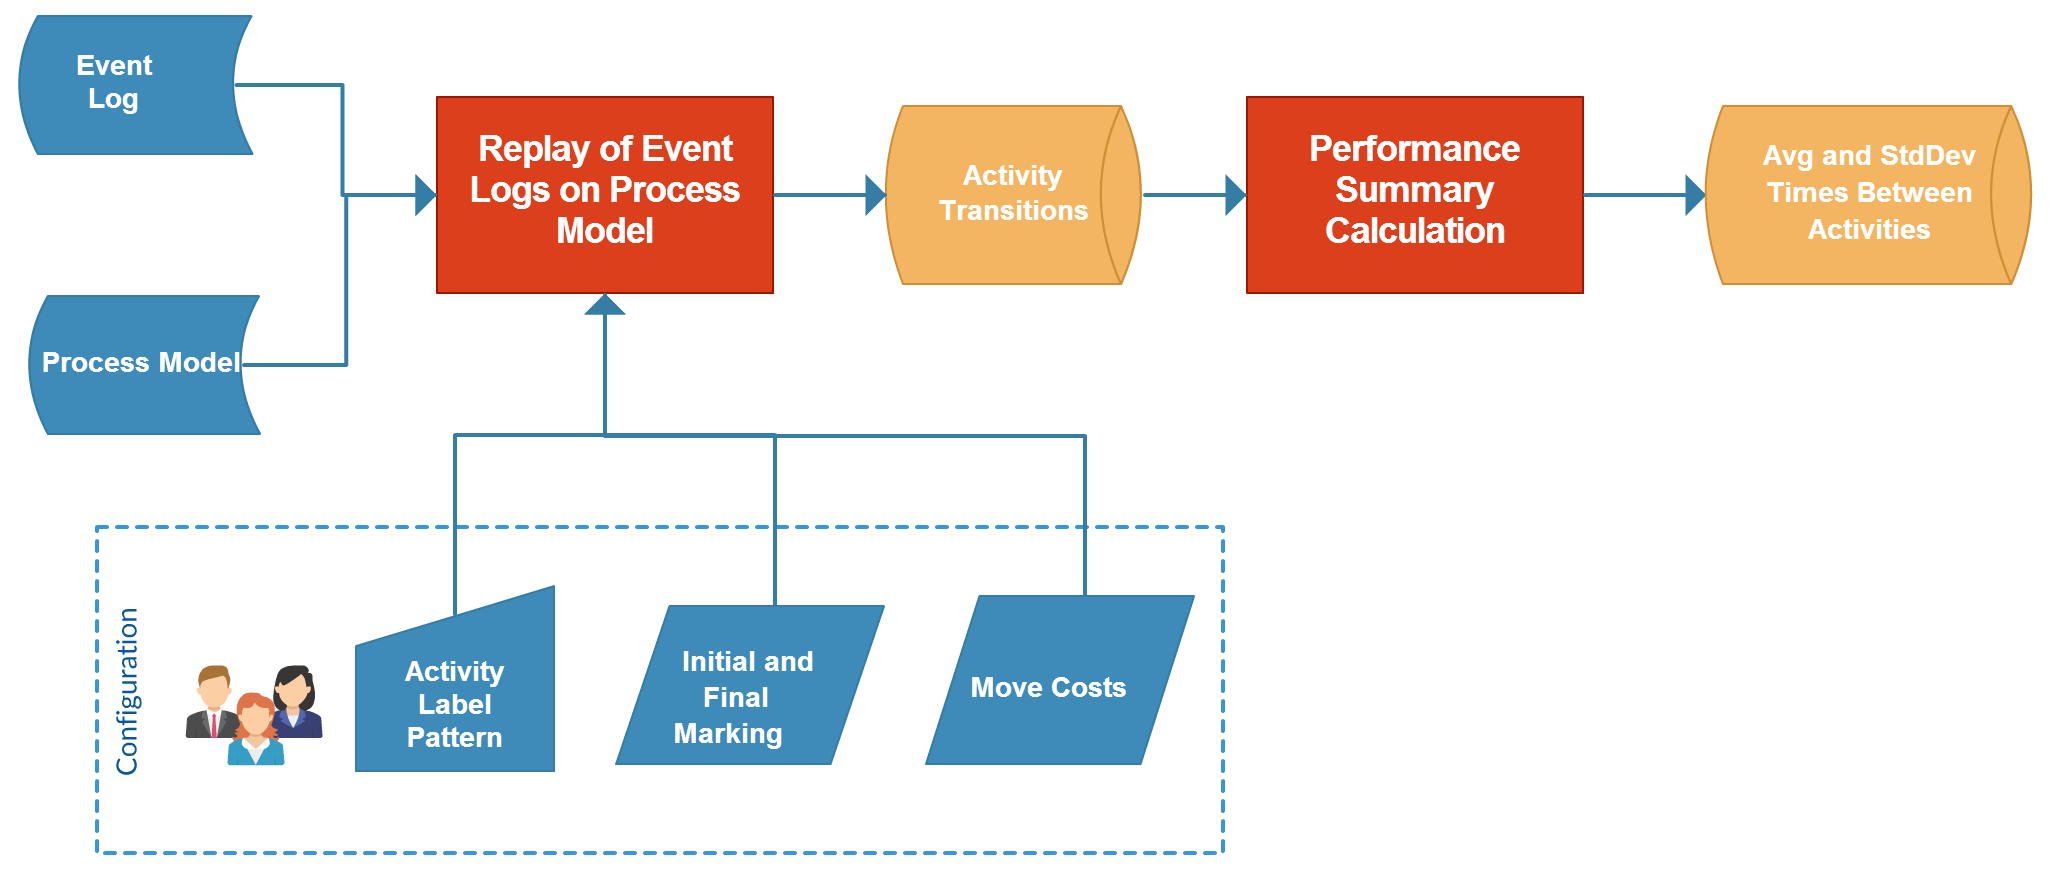
\includegraphics[width=\textwidth]{4_methodology/replay-and-performance-indicator-calculation}
  \caption{Replay and Performance Indicator Calculation Stage as Black-box}
  \label{fig:replay-and-performance-indicator-calculation}
\end{figure}

Performance summary calculation step at the end of this stage is used to create a summary of data consists of average and standard deviation of time between activities. Resulting data can be defined as following:



\subsection{Performance Indicator Clustering}
\label{subsec:performance-indicator-clustering}

kmeans öv

quality of clustering yaz

 
öncelikle performance summary merge & clean 
her i için clustering yapılıyor 
kullanıcıya cluster size seçtiriliyor

Blackbox olarak çiz
	

\section{Mismatch Pattern Analysis}
\label{sec:mismatch-pattern-analysis}
BPMN Conversion
Her biri için tek tek algoritma yazılabilir


\section{Recommendation Generation}
\label{sec:recommendation-generation}



\section{Implementation in ProM Framework}
\label{sec:implementation}
buraya arch. çiz